\documentclass[a4paper,12pt]{article} 

%%% Работа с русским языком
\usepackage{cmap}					% поиск в PDF
\usepackage{mathtext} 				% русские буквы в фомулах
\usepackage[T2A]{fontenc}			% кодировка
\usepackage[utf8]{inputenc}			% кодировка исходного текста
\usepackage[english,russian]{babel}	% локализация и переносы

%%% Дополнительная работа с математикой
\usepackage{amsmath,amsfonts,amssymb,amsthm,mathtools, gensymb} % AMS
\usepackage{icomma} % "Умная" запятая: $0,2$ --- число, $0, 2$ --- перечисление

%%Таблица
\usepackage[table,xcdraw]{xcolor}
\usepackage{caption}
\usepackage{subcaption}
\usepackage{floatrow}
\floatsetup[table]{capposition=top}
\floatsetup[wrapfigure]{capposition=bottom}
%multi-column
%\usepackage{multi-column}
%multi-row
\usepackage{multirow}


%% Номера формул
\mathtoolsset{showonlyrefs=true} % Показывать номера только у тех формул, на которые есть \eqref{} в тексте.

%% Шрифты
\usepackage{euscript}	 % Шрифт Евклид
\usepackage{mathrsfs} % Красивый матшрифт

%% Свои команды
\DeclareMathOperator{\sgn}{\mathop{sgn}}

%% Перенос знаков в формулах (по Львовскому)
\newcommand*{\hm}[1]{#1\nobreak\discretionary{}
{\hbox{$\mathsurround=0pt #1$}}{}}

%% Стиль страницы
\usepackage{fancyhdr}

%% Для рисунков
\usepackage{graphicx}
\usepackage[export]{adjustbox}
\usepackage{float}
\usepackage{ragged2e}
\usepackage{wrapfig}

%Отступы и поля 
\textwidth=20cm
\oddsidemargin=-2cm
\topmargin=-2cm
\textheight=25cm

\pagestyle{fancy}
\begin{document}
\begin{titlepage}
\begin{center}
%\vspace*{1cm}
\large{\small ФЕДЕРАЛЬНОЕ ГОСУДАРСТВЕННОЕ АВТОНОМНОЕ ОБРАЗОВАТЕЛЬНОЕ\\ УЧРЕЖДЕНИЕ ВЫСШЕГО ОБРАЗОВАНИЯ \\ МОСКОВСКИЙ ФИЗИКО-ТЕХНИЧЕСКИЙ ИНСТИТУТ\\ (НАЦИОНАЛЬНЫЙ ИССЛЕДОВАТЕЛЬСКИЙ УНИВЕРСИТЕТ)\\ ФАКУЛЬТЕТ АЭРОКОСМИЧЕСКИХ ТЕХНОЛОГИЙ}
\vfill
\line(1,0){430}\\[1mm]
%\huge{Лабораторная 2}\\
\huge\textbf{Определение предела прочности в анизотропной пластинке}\\
\line(1,0){430}\\[1mm]
\vfill
\begin{flushright}
\normalsize{Рогозин Владимир}\\
\normalsize{\textbf{Группа Б03-106}}\\
\end{flushright}
\end{center}
\end{titlepage}
\fancyhead[c] {Определение предела прочности в анизотропной пластинке}

\textbf{Цель работы:} 
Знакомство с анизотропными материалами и экспериментальное определение предела прочности в функции угла между осями анизотропии и направлением, под которым вырезан образец.  

\textbf{Теоретические сведения:} 
Среда называется анизотропной, если свойства ее в каждой точке зависят от направления. Анизотропия бывает оптическая, механическая и т.д. В настоящей лабораторной работе определяются пределы прочности образцов, вырезанных из ортотропной пластинки под различными углами к осям анизотропии. В разрывной машине эти образцы доводятся до разрушения, и для каждого из них определяется предел прочности по формулу
\[\sigma_b (\varphi) = \frac{P_M}{S}\] 
где $P_M$ -- наибольшая сила, которую выдержал образец, а $S$ -- площадь сечения образца. Так как предел прочности не очень стабильная величина, $\sigma_b (\varphi)$ определяется как среднее арифметическое по нескольким образцам.

\begin{figure}[H]\label{fig: Razlozhenie E}
    \centering
    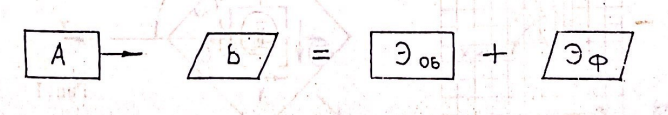
\includegraphics[width=\textwidth]{Разложение энергии.png}
    \caption{Разложение потенциальной энергии}
\end{figure}
Для изотропных материалов можно показать, что потенциальная энергия, накапливаемая в элементарном кубике, может быть представлена в виде суммы: энергии изменения объема и энергии изменения формы. Кубик А после деформации переходит в. Энергия кубика В может быть представлена в виде Эобъём + Эформоизм. 

Энергия формоизменения пропорциональна некоторой квадратичной форме $S$ от компонент напряжений 
\[S^2 = \frac{1}{6} [(\sigma_x - \sigma_y)^2 + (\sigma_x - \sigma_z)^2 + \sigma_y - \sigma_z)^2] + \tau_{xy}^2 + \tau_{xz}^2 + \tau_{yz}^2\]
S называется интенсивностью касательных напряжений. Согласно энергетической теории прочности разрушение материала происходит тогда, когда интенсивность касательных достигает предельного значения. В случае одноосного напряжения разрушение происходит при $\sigma_x = \sigma_b$, то есть
\[S_{разр} = \frac{1}{\sqrt{3}} \sigma_b\]

Для плоского напряженного состояния имеем 
\[S^2 = \frac{1}{3} [\sigma_x^2 + \sigma_y^2 - \sigma_x \sigma_y] + \tau_{xy}^2\]

Можно предположить, что для анизотропных материалов существует аналогичная величина, которую можно назвать обобщённой интенсивностью напряжений, которая также должна быть некоторой квадратичной формой от компонент тензора напряжений
\[S^2 = A\sigma_x^2 + B\sigma_y^2 + C\sigma_x\sigma_y + D \tau_{xy}^2\]
где $\sigma_x$, $\sigma_y$, $\tau_{xy}$  -- компоненты тензора напряжений в осях анизотропии, $A$, $B$, $C$ и $D$ -- постоянные, зависящие от модулей в законе Гука для анизотропных материалов и от текучести, которые для анизотропного материала зависят от направления. В системе координат, где базисные вектора направлены по ортотропным направлениям значения напряжений записываются в виде 
\[\sigma_x = \sigma (\varphi) \cos^2{\varphi}, \quad \sigma_y = \sigma (\varphi) \sin^2{\varphi}^2, \quad \tau_{xy} = \sigma (\varphi) \cos{\varphi} \sin{\varphi}\]
в момент разрушения $\sigma (\varphi) = \sigma_b (\varphi)$. С помощью этих выражений получим значение предельного напряжения.
\[\sigma_b (\varphi) = \frac{S_m}{A\cos^4{\varphi} + B\sin^4{\varphi} + (C + D)\sin^2{\varphi}\cos^2{\varphi}}\]

Построим наилучшую кривую зависимости относительного предельного напряжения от угла
\[\frac{\sigma_b (\varphi)}{\sigma_b (0)} = \frac{\chi}{\chi \cos^4{\varphi} + \sin^4{\varphi} + b \sin^2{\varphi}\cos^2{\varphi}}\]
П

\textbf{Обработка данных:} 
Толщина каждой из пластинок  одна и та же и равна $d = 2$ мм. Ниже в таблице приведены результаты измерений.

\begin{table}[H]\label{tab: Data}
    \centering
    \begin{tabular}{|c|cc|cc|cc|}
        \hline
        {\color[HTML]{000000} } &
          \multicolumn{2}{c|}{{\color[HTML]{000000} I серия измерений}} &
          \multicolumn{2}{c|}{{\color[HTML]{000000} II серия измерений}} &
          \multicolumn{2}{c|}{{\color[HTML]{000000} III серия измерений}} \\ \hline
        {\color[HTML]{000000} $\varphi$, град} &
          \multicolumn{1}{c|}{{\color[HTML]{000000} $b$, мм}} &
          {\color[HTML]{000000} $P_{крит}$,} &
          \multicolumn{1}{c|}{{\color[HTML]{000000} $b$, мм}} &
          {\color[HTML]{000000} $P_{крит}$,} &
          \multicolumn{1}{c|}{{\color[HTML]{000000} $b$, мм}} &
          {\color[HTML]{000000} $P_{крит}$,} \\ \hline
        {\color[HTML]{000000} 0} &
          \multicolumn{1}{c|}{{\color[HTML]{000000} 23,2}} &
          {\color[HTML]{000000} 241} &
          \multicolumn{1}{c|}{{\color[HTML]{000000} 22,8}} &
          {\color[HTML]{000000} 1977,9} &
          \multicolumn{1}{c|}{{\color[HTML]{000000} 21,6}} &
          {\color[HTML]{000000} 1858,7} \\ \hline
        {\color[HTML]{000000} 15} &
          \multicolumn{1}{c|}{{\color[HTML]{000000} 21,8}} &
          {\color[HTML]{000000} 218} &
          \multicolumn{1}{c|}{{\color[HTML]{000000} 22,4}} &
          {\color[HTML]{000000} 1754,3} &
          \multicolumn{1}{c|}{{\color[HTML]{000000} 22,8}} &
          {\color[HTML]{000000} 1923,3} \\ \hline
        {\color[HTML]{000000} 30} &
          \multicolumn{1}{c|}{{\color[HTML]{000000} 21,3}} &
          {\color[HTML]{000000} 186} &
          \multicolumn{1}{c|}{{\color[HTML]{000000} 22,0}} &
          {\color[HTML]{000000} 1434,5} &
          \multicolumn{1}{c|}{{\color[HTML]{000000} 23,2}} &
          {\color[HTML]{000000} 1599,1} \\ \hline
        {\color[HTML]{000000} 45} &
          \multicolumn{1}{c|}{{\color[HTML]{000000} 21,7}} &
          {\color[HTML]{000000} 175} &
          \multicolumn{1}{c|}{{\color[HTML]{000000} 22,5}} &
          {\color[HTML]{000000} 1352,3} &
          \multicolumn{1}{c|}{{\color[HTML]{000000} 21,9}} &
          {\color[HTML]{000000} 1127,2} \\ \hline
        {\color[HTML]{000000} 60} &
          \multicolumn{1}{c|}{{\color[HTML]{000000} 21,6}} &
          {\color[HTML]{000000} 164} &
          \multicolumn{1}{c|}{{\color[HTML]{000000} 22,2}} &
          {\color[HTML]{000000} 1064,9} &
          \multicolumn{1}{c|}{{\color[HTML]{000000} 23,8}} &
          {\color[HTML]{000000} 1387,6} \\ \hline
        {\color[HTML]{000000} 75} &
          \multicolumn{1}{c|}{{\color[HTML]{000000} 21,0}} &
          {\color[HTML]{000000} 152} &
          \multicolumn{1}{c|}{{\color[HTML]{000000} 22,1}} &
          {\color[HTML]{000000} 1026,2} &
          \multicolumn{1}{c|}{{\color[HTML]{000000} 22,8}} &
          {\color[HTML]{000000} 1261,3} \\ \hline
        {\color[HTML]{000000} 90} &
          \multicolumn{1}{c|}{{\color[HTML]{000000} 22,6}} &
          {\color[HTML]{000000} 166} &
          \multicolumn{1}{c|}{{\color[HTML]{000000} 22,1}} &
          {\color[HTML]{000000} 936,0} &
          \multicolumn{1}{c|}{{\color[HTML]{000000} 22,6}} &
          {\color[HTML]{000000} 1151,6} \\ \hline
    \end{tabular}
    \caption{Значения критического напряжения в зависимости от угла}
\end{table}
Для каждого угла усредним значение относительного напряжения разрыва, построим точки на графике. Затем найдём значения параметров $\chi$ и $b$, при которых кривая лучше всего описывает усреднённые точки. Построим эту кривую на том же графике.

\begin{figure}[H]\label{fig: Graph sigma / sigma (phi)}
    \centering
    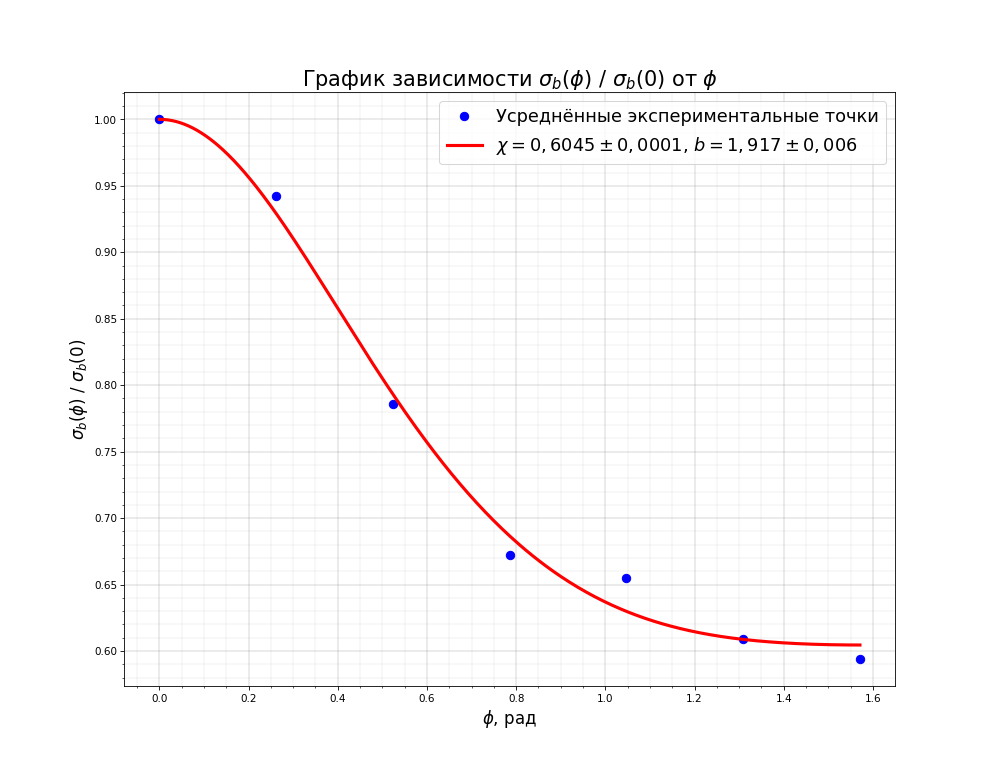
\includegraphics[width = \textwidth]{Финальный график.png}
\end{figure}

%\textbf{Вывод:} 

\end{document}
